\documentclass{article}


\usepackage{kr}

\usepackage{graphicx}
\usepackage{amsmath}
\usepackage{natbib}
\usepackage{xcolor}
\usepackage{amssymb}
\usepackage{amsmath}
\usepackage{subcaption}
\usepackage{algorithm}
\usepackage{algpseudocode}
\bibliographystyle{kr}
\usepackage{hyperref}


\usepackage{rotating}
\usepackage{tikz}
\usepackage{multicol}
\graphicspath{{../figs/}}
\newtheorem{proof}{Proof}
\newtheorem{lemma}{Lemma}



\title{Sequential Cognition Processes: A Framework For Reasoning with Non-Monotonic Logics\\
\large{Mater's Thesis}}
% Single author syntax
\author{%
    Axel Ind
    \affiliations
    Albert-Ludwigs-Universit{\"a}t Freiburg
    \emails
    axeltind@gmail.com    % email
}

\begin{document}

\maketitle

\begin{abstract}
Approaches to cognitive modelling with non-monotonic logics have thus far been largely \textit{ad hoc} and poorly standardised, making inter-model comparisons difficult. As an attempt to systematically represent non-monotonic logics in a framework that standardises cognitive modelling under these logics without sacrificing their expressiveness, we introduce the Sequential Cognition Process (SCP). Under the assumption that human reasoning can be represented as a sequence of distinct cognitive operations on an initial knowledge base SCPs provide a consistent framework for generating and evaluating models of human cognition. Using an adapted interpretation of the Weak Completion Semantics (WCS), SCPs are able to accurately model several classical experiments in cognitive modelling. We use the SCP framework to model both general case reasoners -- which arrive at the most frequently observed conclusions -- and poorly-studied individual case reasoners -- which do not. We illustrate the use of SCPs using the Suppression Task.
\end{abstract}

\section{Introduction}
\subsection{Overview}
% a statement of the problem
\subsection{A Review of Terminology}
% a review of terms
\subsection{Current State of the Art}
% review of literature
\subsection{Contributions of the SCP Framework}
\subsection{Thesis Layout}
% description of remaining chapters

\section{Mathematical Preliminaries}
\subsection{Logic Programming}
\subsection{The Weak Completion Semantics}
\subsection{Reiter's Default Logic}


\section{Experiments}

\section{Sequential Cognition Processes}
\subsection{SCPs: An Intuitionist Description}
\subsection{SCPs: Mathematical Formulation}
\subsection{Overview}
\subsection{SCPs vs SCP Tasks}
\subsection{Epistemic States}
\subsection{State Points}
\subsection{Pre-conditions and Effects}
\subsection{The Categorization Variable}
\subsection{Search in SCP-Space}
\subsubsection{De-Novo SCP Searching}
\subsubsection{Insertion Search}

\section{Comparing SCPs}
\subsection{Why do we need to compare SCPs?}
\subsection{Comparing Generated SCPs}
\subsection{Comparing External SCPs}
\subsubsection{The Needleman-Wunsch Algorithm}
\subsubsection{A Modified Scoring Algorithm}


\section{Program Design}
\subsection{Implementing the SCP Framework}
\subsection{A Modular Programming Approach}
% talk about each 




\section{Non-Sequential Cognitive Processes}
% relation to neural networks
% summarising tool



\section{Conclusions and Future Work}
\subsection{Conclusion}
\subsection{Future Work}

\section*{Appendix}














\section{Introduction}
The human mind is complex. So complex that thousands of approaches from dozens of fields have failed to capture its complexity. The sheer size of the brain -- containing  over 5000 times as many neurons as the largest practical neural networks \citep{mocanu2018scalable} -- and our limited understanding of the fundamental learning processes it employs mean that researchers can neither completely describe nor predict human actions nor model human thought processes. Instead, much of the current state of the art in cognitive modelling relies on one of two general approaches: creating systems that structurally approximate the human brain, and creating systems which approximate a more abstract intuition of cognition. The first type of system encompasses many algorithms related to machine learning and deep learning; the second type, with which this paper is concerned, has existed in some form for far longer than humans have been thinking creatures \citep{smirnova2015crows}. Every shark stalking its prey, every tiny proto-mammal hiding from a hungry dinosaur, and every man driving to work in the morning, has applied this type of reasoning when trying to make predictions about the actions of other agents in their world. By applying case-specific reasoning to a known world state we are able to make imperfect, but quick, predictions about the mental state of other agents in our world.

Due in part to the difficulty of cloning dinosaurs to hunt participants in cognitive research experiments, and partly due to concerns about the ease with which they could answer questionnaires on the experience later, most cognitive tasks used by researchers tend to be more dull than the examples above.

Non-monotonic logics have proven able to adequately model a large number of standard cognitive reasoning tasks such as The Wason Selection Task\citep{wason1968reasoning} and Suppression Task \citep{byrne1989suppressing}. These approaches, though effective and well-founded in isolation, are often unable to integrate or be compared to data models of other tasks, even when they rely on the same underlying logic. Although the non-monotonic logics themselves are generally carefully described, procedures ranging from best practise in deciding appropriate knowledge bases to the mechanisms by which abnormalities should be created tend to be re-imagined on a case-by-case basis.

Further, cognitive frameworks using non-monotonic logics are almost always designed to describe the most common (general) conclusion drawn by participants in the experiment. Modelling other individual reasoners or classes of reasoners who differ from the norm is often a non-trivial process. It has been shown that the Weak Completion Semantics \citep{holldobler2015weak} is able model the four most general cases of the Wason Selection Task under the assumption that reasoners who differ from the general case (\textit{deviant reasoners}) follow a sequence of mental processes that is still highly similar to that of the general reasoner \citep{breu2019weak}.

This paper introduces the Sequential Cognition Process (SCP) which generalises the assumption of sequential cognitive operations, each of which uses a collection of epistemic states as input and produces a collection of epistemic states as output. Using SCPs and a set of well-founded cognitive operations it is possible to apply traditional search techniques to problems in cognitive modelling with non-monotonic logics that have previously required expert-made models. The SCPs introduce a number of desirable properties: they introduce a partially standardised (though extensible) set of allowable cognitive operations, they standardise the structure of what constitutes an epistemic state, they are easily modified to accommodate deviant reasoners when a well-founded general model already exists, and their sequential structure makes them well-suited to scoring algorithms that allow intra- and inter-experimental modelling and comparisons.

Section~\ref{sec:matPrem} introduces the mathematical background necessary to understand the SCP framework when it is used in the context of non-monotonic logics in general and the WCS in particular. Section~\ref{sec:sup} introduces one common formulation of the Suppression Task and shows how the WCS has been used to model the most common (general) inference drawn by participants. Section~\ref{sec:scp} introduces the SCP framework from both an intuitive and a mathematical sense, as well as addressing the concept of the epistemic states in some detail. Section~\ref{sec:mod} provides a concrete illustration of the use of SCPs by modelling both the general case of the Suppression Task as well as an individual case for those who do not draw the most common inferences. Finally, Section~\ref{sec:conc} summarises the key contributions of this paper and proposes several possible research questions related to the SCP framework.


\section{Mathematical Preliminaries}\label{sec:matPrem}
Before discussing the WCS, it is important to understand why non-monotonic logics are required for cognitive modelling at all. There are a number of empirical studies demonstrating that humans consistently fail to draw the classically valid conclusions to certain cognitive tasks \citep{byrne1989suppressing}, \citep{wason1968reasoning}. Section~\ref{sec:sup} describes the Suppression Task, in which human test subjects repeatedly make the classically invalid inference that, given some knowledge base $KB$, it is possible for $KB \models \phi$ to be true, but $(KB \cup \psi) \models \phi$ to be false.

\subsection{Propositional Logic}

\begin{table}
\begin{center}


\begin{tabular}{ c | c c }
  $\land$& $\top$ & $\bot$ \\ \hline
 $\top$ & $\top$ & $\bot$ \\  
 $\bot$ & $\bot$ &  $\bot$
\end{tabular}
\quad
\begin{tabular}{ c | c c }
  $\lor$& $\top$ & $\bot$ \\ \hline
 $\top$ & $\top$ & $\top$ \\  
 $\bot$ & $\top$ &  $\bot$
\end{tabular}
\quad
\begin{tabular}{ c | c }
  $\lnot$& \\ \hline
 $\top$ & $\bot$ \\  
 $\bot$ & $\top$
\end{tabular}

\begin{tabular}{ c | c c }
  $\rightarrow$& $\top$ & $\bot$ \\ \hline
 $\top$ & $\top$ & $\bot$ \\  
 $\bot$ & $\top$ &  $\top$
\end{tabular}
\quad
\begin{tabular}{ c | c c }
  $\rightarrow$& $\top$ & $\bot$ \\ \hline
 $\top$ & $\top$ & $\bot$ \\  
 $\bot$ & $\bot$ &  $\top$
\end{tabular}

\caption{Truth tables for standard operators in propositional logic.}
\label{tbl:prop}

\end{center}
\end{table}

Propositional (or classical) logic is the form of logic most traditionally associated with problem solving in mathematics and computer science. In propositional logic features of a hypothetical world are encoded by a set of \textit{variables}. every variable must be mapped to either $\top$ (usually denoting truth, in some subject-specific sense) or $\bot$ (denoting falseness). A \textit{clause} $\phi$ consists of either a single atomic variable or an operator and some set of sub-clauses. Every clause has a truth value determined by the values of the sub-clauses it contains and the relevant operator which handles their interaction. Table~\ref{tbl:prop} illustrates the classical interpretations of the allowable operators. A knowledge base $KB$ consists of a set of clauses. In this paper we adopt the assumption all clauses (also called rules) $\in KB$ are of the form $head\leftarrow body$ and all heads are atomic variables.

\subsection{Non-monotonic Logics in General}
In the field of non-monotonic logics, reasoning is represented as a collection of defeasible inferences. Unlike in classical logic, conclusions need not hold in perpetuity, or even in the same model and revision is always possible. Monotonic logics are not capable of describing human reasoning in experiments like the Suppression Task \citep{dietz2012computational} because they lack this revisionist characteristic.

A large number of non-monotonic frameworks exist in the literature \citep{mcdermott1980non}, each applicable to a different subset of cognitive problem space, and each modelling their problem space with various degrees of success. In the simplest formulation, a non-monotonic logic is simply an extension to a classical logic which introduces a preference relation $\rightarrow_p$. This preference relation states that, given some number of derivable facts in a knowledge base, the fact derived using the most preferential rule is to be derived first and cannot be overwritten by a less preferable assignment.  


\subsection{The Weak Completion Semantics} \label{ssec:wcs}

\begin{table}
\begin{center}
\begin{tabular}{ c | c c c }
  $\rightarrow$& $\top$ & $u$ & $\bot$ \\ \hline
 $\top$ & $\top$ & $u$ & $\bot$ \\  
 $u$ & $\top$ & $\top$ & $u$\\  
 $\bot$ & $\top$ & $\top$ & $\top$
\end{tabular}
\caption{A table showing the implication operator in 3-valued \L ukasiewicz logic.}
\label{tbl:luk}
\end{center}
\end{table}

The Weak Completion Semantics is a non-monotonic logic which procedurally encodes several well-known cognitive phenomena. The WCS makes use of 3-valued \L ukasiewicz logic (Table~\ref{tbl:luk}). It adds abnormalities to non-ground inferences, and replaces the classical inference ($\leftarrow$), with a bijective ($\leftrightarrow$). 

The Weak Completion of a program $P$ is defined as follows:

\begin{enumerate}
\item Replace all clauses of the form $A \leftarrow body_1$, ..., $A \leftarrow body_n$ with $A \leftarrow body_1 \lor ... \lor body_n$.
% \item For all undefined variables $x$, add $x \leftarrow \bot$. THIS IS FOR STRONG COMPLETION ONLY
\item Replace all occurrences of $\leftarrow$ with $\leftrightarrow$.
\end{enumerate}

Applying this procedure to $P$ results in $wcP$ which is the weak completion of $P$.

The next requirement to apply the WCS framework is the introduction of a semantic operator $\phi_{SvL}$ \citep{stenning2008interpretation}. Let $J$ be the result of applying the semantics operator to an interpretation $I$ and logic program $P$. Then $J$ is defined as follows:

\[
\begin{split}
J^\top = \{ & A | \textrm{ there exists a clause } A\leftarrow Body \in P \\ & \textrm{ with } I(Body) = \top\}
\end{split}
\]
\[
\begin{split}
J^\bot = \{ &  A | \textrm{ there exists a clause } A \leftarrow Body \in P \\
           & \textrm{ and for all clauses } A \leftarrow Body \in P \\ & \textrm{ we find } I(Body) = \bot\}
\end{split}
\]

%this might not be right? Should it say I or J? @TODO
Using $I=<\emptyset, \emptyset>$, the least model of $P$ ($\textrm{lm}_\textrm{\L}$wc$P$) can be calculated by iterating $\phi_{SvL,P}$.

\section{Experiments: The Suppression Task} \label{sec:sup}
The Suppression Task refers to an experiment conducted by \cite{byrne1989suppressing} and is a classical example of the inadequacy of monotonic logics for modelling human reasoning. In classical logic, if our knowledge base $kb$ is such that $kb \models \phi$, then it must be the case that $kb \cup \psi \models \phi$. However, in the suppression task participants no longer draw classically valid inferences when new information is added. The task is often formulated as follows:

\begin{itemize}
\item $e \rightarrow l$: If she has an essay to write ($e$), she will study late in the library ($l$).
\item $\top \rightarrow e$: She has an essay to write ($e$).
\item $o\rightarrow l$: If the library is open ($o$), she will study late in the library ($l$).
\end{itemize}

Given only the rules $(e \rightarrow l)$ and $(\top \rightarrow e)$, the participants consistently concluded that she would study late in the library, seemingly drawing the classical logic inference $\frac{e \rightarrow l, e}{l}$ with \textit{modus ponens}. But when given the additional rule $o\rightarrow l$, participants no longer believe that they have enough information to judge whether she will study late in the library, and a significant portion of them no longer draw the classical conclusion. This effect, called Suppression, demonstrates the need for something more than classical logic for modelling human reasoning.

Work by \cite{dietz2014modeling} has shown that the WCS is an adequate non-monotonic logic for modelling the Suppression Task. Under the WCS and \L ukasiewicz 3-valued logic the task is usually modelled as follows for the case without suppression:
\begin{enumerate}
\item Initial logic program: $P = \{e \rightarrow l, \top \rightarrow e \}$. This program represents the task without information about what happens if the library is open.
\item Addition of Abnormality: $P = \{e \land \lnot ab_1 \rightarrow l, \top \rightarrow e, \bot \rightarrow ab_1 \}$. The program now reflects the possibility that some abnormal event may prevent her from going to the library, but because we have no information about the nature of this event, it is set to false by default.
\item Weak Completion: $wc(P) = \{e \land \lnot ab_1 \leftrightarrow l, \top \leftrightarrow e, \bot \leftrightarrow ab_1 \}$. Weak completion is applied to the logic program and, in this case, only implications need to be changed to bijections.
\item Semantic Operator:
\begin{itemize}
\item Execution 1: $\top=\{e\}, \bot=\{ab_1\}$
\item Execution 2: $\top=\{e,l\}, \bot=\{ab_1\}$
\end{itemize}
\end{enumerate}

After application of the semantic operator $l$ is true in the least model, and so participants conclude that she will study late in the library (as when $P$ is evaluated classically). However, in the case where Suppression is observed, the same process yields a different result because of the presence of the extra conditional ($o\rightarrow l$).
\begin{enumerate}
\item Initial logic program: $P = \{e \rightarrow l, \top \rightarrow e, o \rightarrow l \}$. The initial program now includes information about the extra (suppressing) conditional.
\item Addition of Abnormality: $P = \{e \land \lnot ab_1 \rightarrow l, o \land \lnot ab_2 \rightarrow l, \top \rightarrow e, \lnot o \rightarrow ab_1, \lnot e \rightarrow ab_2 \}$. An abnormality $ab_i$ is an addition to an inference which captures the idea that external factors may invalidate the conclusion of the original inference. Adding abnormalities is a poorly described process and often relies on intuitionist views of what actually constitutes an abnormal situation. In this case we adopt the practise of identifying abnormalities as described in Appendix~\ref{ssec:addAbnormalities}.
\item Weak Completion: $wc(P) = \{((e \land \lnot ab_1) \lor (o \land \lnot ab_2)) \leftrightarrow l, \top \leftrightarrow e, \lnot o \leftrightarrow ab_1, \lnot e \leftrightarrow ab_2 \}$. Weak completion is applied to the logic program, combining rules with shared heads and replacing implications with bijections.
\item Semantic Operator:
\begin{itemize}
\item Execution 1: $\top=\{e\}, \bot=\{ab_2\}$
\end{itemize}
\end{enumerate}

Now suppression has been displayed in the logic program and the variable $l$ remains unknown in the least model.

\section{Sequential Cognition Process} \label{sec:scp}
\subsection{SCPs: an Intuitive Description}
\begin{figure*}
\begin{subfigure}{.35\textwidth}
  \centering
  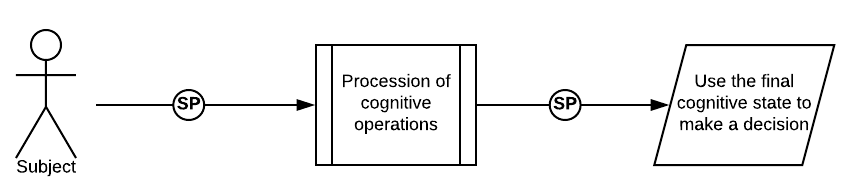
\includegraphics[width=0.97\linewidth]{general}
  \caption{Unrestricted SCP.}
  \label{fig:scp_general}
\end{subfigure}%
\begin{subfigure}{.65\textwidth}
  \centering
  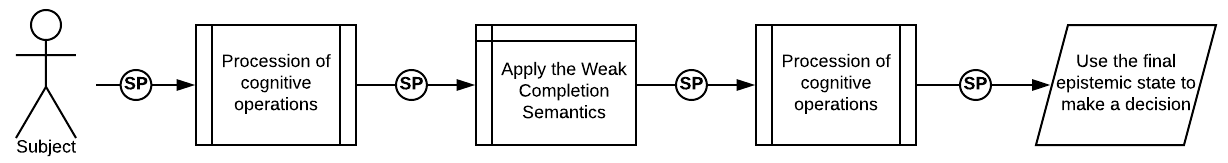
\includegraphics[width=0.97\linewidth]{generalWCS}
  \caption{WCS guaranteed to occur.}
  \label{fig:sfig2}
\end{subfigure}
\caption{The most general description on an SCP with and without guaranteeing the WCS is applied at least once. An agent transitions from one epistemic state to another and then uses it to make a decision. $SP$ nodes indicate state points.}
\label{fig:scp_generalWCS}
\end{figure*}

Although there is evidence that the brain can perform several simultaneous operations when considering a task (such as when considering an image \citep{sigman2008brain}, the SCP framework assumes that at some points in reasoning about a given task, the mental processes of the agent converge to a set of epistemic states, called a \textit{state point}. Whatever happens between these points of convergence can contain any number of parallel processes. The collection of processes that occur between any two state points in a reasoning task is called a \textit{cognitive operation}. It follows that any cognitive operation is valid as long it takes a set of epistemic states as input and produces a set of epistemic states as output. Figure~\ref{fig:scp_general} describes an SCP that is powerful enough to model any cognitive task that involves an epistemic state transition. However, it does not provide any useful information; the nature of the processes followed is completely undescribed. Suppose, instead, that some cognitive task is being modelled, and that researchers have reason to believe that The Weak Completion Semantics should play a part in their model. Under this new restriction, and assuming a sufficiently expressive epistemic state, Figure~\ref{fig:scp_general} is still an accurate model of the process, but now so is Figure~\ref{fig:scp_generalWCS}. By sacrificing some of the ambiguity -- and, thus, expressiveness -- of the model, the information content of the model description has increased. This trade-off is a feature of the SCP framework and finding the right depth of complexity to model the task accurately and still provide meaningful information is more art than science at present. 

\subsection{SCPs: a Formal Framework}
An SCP Task $\Pi=(s_i, \gamma, M)$ consists of an initial epistemic state $s_i$, known goal state $\gamma$, and a known set of cognitive operations $M$. An epistemic state $s_k$ describes all the information available to the agent at state point $k$. The precise contents of an epistemic state should be chosen so that at least some $m \in M$ are able to accept that state as an input. In the case of a system containing only the one complex operation which applies the WCS, one possible epistemic state is $s=(KB,V)$, where $KB$ describes a knowledge base consisting only of rules of the $(head \leftarrow body)$ and $V$ is a mapping of atom names appearing in $KB$ to a truth value in \L ukasiewicz logic ($\top,u, \bot$). In principle this definition will serve for the rest of the paper, but it is extended slightly so that $s_k = (KB,V,R)$ where $R$ is a set of labelled categorization criteria sets (\textit{LCS}). An LCS $ c \in R$ consists of a category name and list of rules and atoms which fit into that category.

A base point is a single epistemic state. A state point $p$ is defined recursively by $p=\{\bar{p} \oplus Q \}$ where $\bar{p}$ is a base point, and $Q$ is a set of state points, and $\oplus$ represents the exclusive-or operation\footnote{$(X \oplus Y) = ((X \cup Y) - (X \cap Y))$ for sets $X$ and $Y$.}. State point containment $\in_s$ for state points $p$ and $q$ is defined recursively as follows:

\[
p \in_s q = \begin{pmatrix} p \in q  & \textrm{True} \\ p \not\in q \textrm{ and } q \textrm{ is a base point} & \textrm{False}  \\  \exists_{r\in p}p \in_s r = \textrm{True} & \textrm{True}   \\ \textrm{Otherwise} & \textrm{False} \end{pmatrix}
\]

It is never the case that $p \in_s p$.

A cognitive operation $m = (\chi, e), m \in M$ consists of a precondition $\chi$ and a process $e$, such that for an input state point $p$, every base point $\bar{p} \in_s p$ is either accepted as input ($\bar{p} \models m[\chi]$ under whatever definition of $\models$ is used for the complex operation $m$), or else rejected. Every base point is evaluated by the complex operation in isolation (no other base point $\bar{q}$ can affect the output of $m$ on base point $\bar{p}$). To capture the fact that cognitive operation may utilize non-monotonic logic, applying $m$ to an input base point $\bar{p}\in p$ always yields a state point $p'$ (written $J[\bar{p},m]=p'$) which describes all possible resulting epistemic states that can be generated. 

Applying $m$ to an input state point $p$ is done by replacing every base point $\bar{p} \in p$ with $J[\bar{p},m]$. A cognitive operation is called monotonic if it always yields a base point as an output given a base point input ($J[\bar{p},m]=\bar{p'}$). It follows that the depth of a state point is directly related to the number of complex operations which have been performed in the SCP prior to its occurrence. If a base point does not meet the precondition, it is either ignored completely and not processed (\textit{cruel application}), or passed exactly as is to the next complex operation (\textit{lenient application}). It is worth noting that the type of cognitive states produced as output by $m$ may not be the same as those of the input.

This paper will focus on cases where the type of cognitive state remains constant, but there is no reason in principle that a base point input $s_k = (KB,V,R)$ for the WCS could not be returned as a base point $s_k = (KB,V,R,D)$ where $D$ is a set of default rules usable by cognitive operations that implement Reiter's Default Logic \citep{reiter1980logic}. Future models of human cognition may well rely on background knowledge which draws inferences from multiple types of non-monotonic logics.

An SCP $\pi=(s_i,m_1,...,m_n)$ describes an initial epistemic state (or state point if the input is uncertain) and state point $p_k$ is defined recursively by $p_k = J[p_{k-1},m_k]$. An SCP is called \textit{credulously valid} if $p_n \models \gamma$ for at least one epistemic state in the final state $p_n$. An SCP is called \textit{sceptically valid} if $p_n \models \gamma$ for every epistemic state in the final state. In cases where all operations are monotonic, sceptical validity is the same as credulous validity.


\subsection{Choosing an Epistemic State}
The choice of epistemic state is dependent on the properties that are known or suspected to be true for the cognitive task as a whole. For example, a researcher working on drawing inferences using Propositional Logic can be certain that any SCP they create should be expressive enough to pass a knowledge base to a cognitive operation. Thus, it might suffice to simply define $s_i=(KB)$ where $KB$ is a set of propositional rules. By contrast, a researcher using the WCS requires a system capable of both communicating a set of rules to the next complex operation, and of describing the results of repeated applications of the semantic operator. It might seem intuitive to simply keep the epistemic state used for the propositional case and to use a non-complex operation function on the weakly completed program to find the least model. And, though this approach works for many examples, it makes it impossible to perform further processing in the SCP \textit{after} applying the semantic operator. What if the conclusion drawn was meant to form part of the background knowledge of another process? In practice using $s_k=(KB,V, R)$, where $V$ is a set of (variable name, value pairs) and $R$ is a categorization variable, is able to model all aspects of the WCS, including information related to the least model. 

The final property of a cognitive operation that needs to be discussed is how it is able to interact with the categorization variable $R$. Imagine a case drawn from \cite{saldanha2017weak} where the difference between creating abnormalities for obligate and factual conditionals is discussed. The intuition behind the authors' work can be summarised by saying that there are two different types of conditional statement, those that \textit{have to be} true, and those that are \textit{usually} true. If it rains $r$, I will normally take my umbrella $u$ (in the absence of something abnormal happening, like a plague of umbrella-stealing gnomes). This a statement that is usually true, but some things are definitely true. For example, when it rains, water has to fall out of the sky $s$. This is an essential property of rain, not subject to abnormalities. Thus one useful set of categorizations for researchers seeking cosmic knowledge of weather patterns may be: $R=\{obligate: \{u \leftarrow r\}, factual: \{s \leftarrow r\} \}$. With these labels we might then expect that the process followed by the operation $m \in M$ which creates abnormalities would treat the two conditionals in $KB$ differently, because of their assignments in $R$. $R$ then is a way of expressing meta information to the cognitive operations, and it is completely possible that some operation $m_k$ might change $R$ is such a way that future operation $m_{k+l}$ produces different output. This is a technique we will exploit in several examples in this paper.

As yet, there are no definite rules for creating an epistemic state, but Albert Einstein's famous advice from 1950 still rings true: ``Everything should be made as simple as possible, but no simpler.'' The ideal epistemic state is one that enables every reasonable cognitive operation in $M$ that might help model the problem, without adding superfluous functionality that might render searching the SCP space infeasible.
\subsection{Choosing a set of Complex Operations}
The set of possible complex operations $M$ determines many attributes of the achievable final state point $p_n$. If every $m \in M$ is monotonic, then $p_n$ will be monotonic. If some cognitive operation is computationally complex or produces a very large number of output state points, then search using that base point becomes less efficient. If some complex operation $m'$ (such as weakly completing) is known or believed to occur in the SCP, then a restriction on the cognitive states exists such that either the initial state is of a format suitable as input for $m'$, or there exists another cognitive operation which is able to output a state point which contains base points of a suitable format.

More abstractly, the set of cognitive operations should be well-founded in the literature. The set of possible complex operations is infinite and an SCP only meaningfully describes human cognition when it contains cognitive operations that have been justified empirically (\textit{modus ponens-modus tolens} asymmetry, suppression, denial of the antecedent, etc.). 

\section{Modelling with SCPs} \label{sec:mod}
\subsection{SCPs Under the Weak Completion Semantics}

\subsubsection{The Suppression Task}
\begin{figure*}
\begin{center}
 \centering 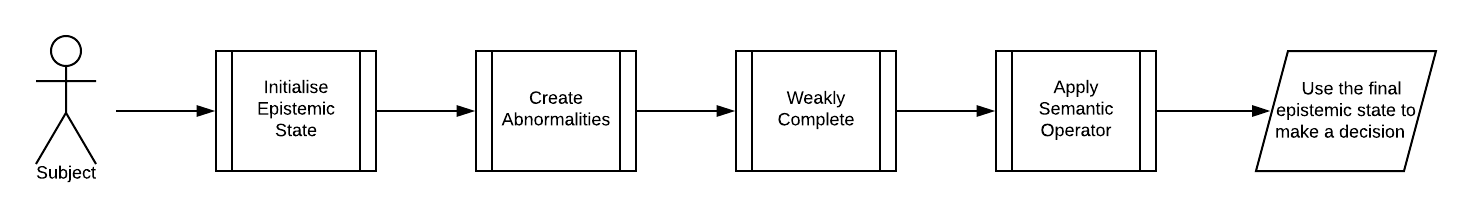
\includegraphics[width=\linewidth]{suppressionSCP_overview}
\caption{A generalised illustration of the WCS in an SCP. }
\label {fig:supoverview}
\end{center}
\end{figure*}

\begin{figure*}
\begin{center}
 \centering 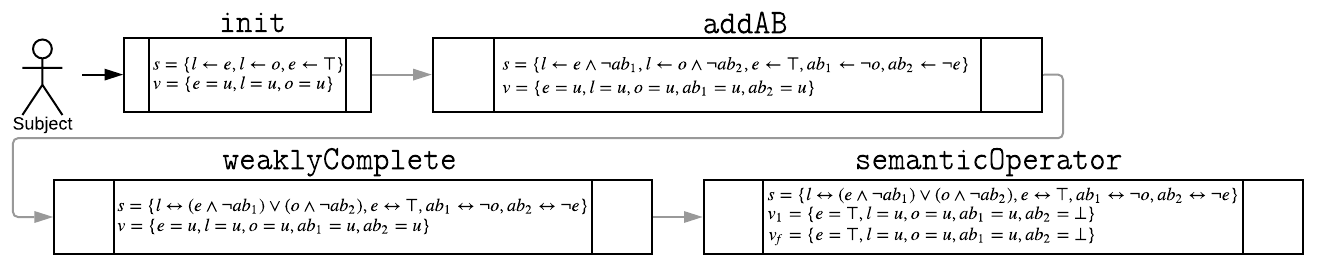
\includegraphics[width=\linewidth]{suppressionSCP_normal}
\caption{The standard case of the Suppression Task, demonstrating the suppression effect. Where the epistemic state in the boxes represents the output of that cognitive operation. $V_f$ represents the assignment of $V$ in the epistemic state in the resulting least model. $V_{i\in \mathbb{N}}$ represents the assignments in $V$ after $i$ iterations of the semantic operator.}
\label {fig:supnormal}
\end{center}
\end{figure*}

Figure~\ref{fig:supoverview} illustrates a generalised SCP to describe the Suppression Task as a series of sequential steps directly mirroring the discrete steps outlined in Section~\ref{sec:sup}, each cognitive operation passing information to the next process\footnote{It is important to note that a diagram like this is valid for \textit{any} cognitive modelling task because any process may be arbitrarily complex and non-sequential. and so the overall linear process of (actor, complex decision, observed results) is always valid for retroactive modelling, and at least as powerful as the non-monotonic logic framework it uses for modelling.}. To model the SCP the implicit sequence of operations in the Suppression Task is systematized and refined into a set of complex operations. Further we introduce an initial epistemic state $s_i=(KB,V,R)$. One interpretation of the requirements of the suppression task $\pi=(s_i,\gamma,M)$ using SCPs and the WCS is as follows: 
 
 
 
 


\[s_i=\{KB_i, V_i, R_i\} \]
\[KB_i=\{e \rightarrow l, \top \rightarrow e, o \rightarrow l\} \]
\[V_i=\{e:u, l:u, o:u\} \]
\[R_i=\{\} \]
\[
\begin{split}
M= \{\texttt{init}, \texttt{addAB}, \texttt{WeaklyComplete},
\\ \texttt{semanticOperator}\}
\end{split}
\]
\[\gamma = (l\models \top) \textrm{ or } (l \models \bot)\]

%@TODO change semanticOper to semanticOperator without line overflowing 

where all cognitive operations require as input and produce as output a state point $p$ where every ground point $\bar{p} \in_s p$ is of format $\bar{p}=(KB,V,R)$; \texttt{init} is always the first cognitive operation and adds the initial variables and rules to epistemic state; \texttt{addAB} adds abnormalities to the current epistemic state using the procedure described in Algorithm~\ref{alg:addAbnormalities} (but now also adds those abnormalities to the variable list of the epistemic state); \texttt{WeaklyComplete} weakly completes the knowledge base of the current epistemic state; and \texttt{semanticOperator} returns an epistemic state that leaves the knowledge base unchanged but updates the variables of that state to return the least model of the epistemic state. \texttt{semanticOperator} follows the same logic seen in Section~\ref{ssec:wcs}, but directly updating $V$ after each iteration of the semantic operator, instead of the externalised variable set $J$. Thus, we ensure that the output state point is able to communicate the result of applying the semantic operator without any structural changes to the epistemic states it contains. As an additional feature of the \texttt{semanticOperator} cognitive operation, if there exists a labelled set in $R$ called $fixed$, then the semantic operator will not set the value of any $v \in fixed$ in the variables list $V$. The goal $\gamma$ states that $l$ should no longer be mapped to unknown in the final epistemic state.



Treating Figure~\ref{fig:supoverview} as an SCP, we observe the sequence of output states seen in Figure~\ref{fig:supnormal}. Note that in the final state $l$ remains mapped to $u$, meaning that the suppression effect is demonstrated.

\subsubsection{Extending the Suppression Task with SCPs}
The previous example merely showed that SCPs are suitable for modelling the suppression task. In this example we consider one of the most powerful characteristics of SCPs, the ability to model unusual results as deviations from general reasoning. In the original Suppression Task Experiment examined in Section~\ref{sec:sup}, a significant portion of people still believed that she would study late in the library, even though the majority suppressed the inference. Several possible explanations are intuitive, the first and simplest, is the assumption that the reasoner is using classical logic and drawing the classical conclusion. However, what if that is not the case? What if they do reason in exactly the same way as the other reasoners, except for one or two small deviations?

In order to model these non-general reasoners, we consider two possible deviations that could explain the classical result of the Suppression Task: \textit{variable deletion}, and\textit{ variable fixation}. Both of these operations will be discussed in a way that may seem overly prosaic, but it is done to reinforce that we might, reasonably, expect these cognitive operations to occur in day-to-day human cognition.

\subsubsection*{Variable Deletion} \label{ssec:variableDeletion}
Consider the sequence of numbers: 1, 44, 27, 8, 0 , -4, 6, 7, 346, 7, 74, 7, 234, -55, 2.4, 18. Now without looking back at the numbers, ask yourself some questions: how many numbers were there? Were any of them prime? How many numbers were repeated? In all probability you are not entirely sure. This simple thought experiment provides support for our first extension, the idea that variables can be ``forgotten", that is, that information that existed in the knowledge base at one point in time might no longer exist at a later timepoint. 

This is not the only imaginable case where a variable might be removed from the knowledge base of the person being modelled. The size of the knowledge base used for cognitive modelling is always implicitly restricted to relevant variables. Only those variables whose values might reasonably be expected to affect the final conclusions drawn with regard to the research question should be considered. Finding which variables and rules are relevant is, however, non-trivial. For another real-life example, imagine a mystery novel: Three hundred pages of plot descriptions, character actions, and dialogues. In a good murder mystery novel every piece of information that reveals the killer's identity is hidden in the story itself, yet we do not hold every fact and interaction in the book in our epistemic model of the book, so discerning the identity of the killer remains a mystery until the last page. But when the mystery is solved, many details that we internalised while reading (and recall in retrospect) suddenly make the conclusion seem obvious. We have not forgotten this information, we had merely incorrectly deemed it irrelevant at the time and ignored it in our cognitive processing.

The exact details of how to delete a variable from a knowledge base are non-trivial, and there is no best practice for doing so. But in simple cases the process can be intuitive. Let \texttt{delete} be a complex operation. \texttt{delete} takes as input any state point and is applicable for any ground point $\bar{p}$ with variable list $V \in \bar{p}$ and categorization variable $R$ with ($delete:V_{del}) \in R$, where $V_{del}$ is the set of variable names to delete. For every $v \in V_{del}$ remove all rules from $KB$ that have $v$ as body or head of the clause, and remove $v$ from $V$. Then remove $delete$ from $R$.

In the case of the Suppression Task we argue that one cognitively valid reason for drawing the classical conclusion to the task may be forgetting (or disregarding) the variable $o$. Figure~\ref{fig:supmod} illustrates this case, and shows how the insertion of a complex operation can completely change the final epistemic state.

\begin{figure*}
\begin{center}
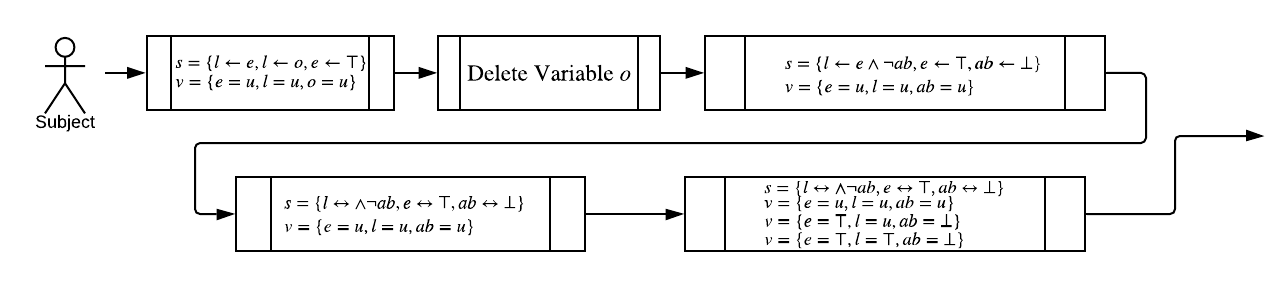
\includegraphics[width=0.85\linewidth]{suppressionSCP_mod}
\end{center}

\caption{The Suppression Task in which the additional operation of deleting the variable $o$ occurs.}
\label{fig:supmod}
\end{figure*}

\subsubsection*{Variable Fixing} \label{ssec:variableFixing}

\begin{figure*}
\begin{center}
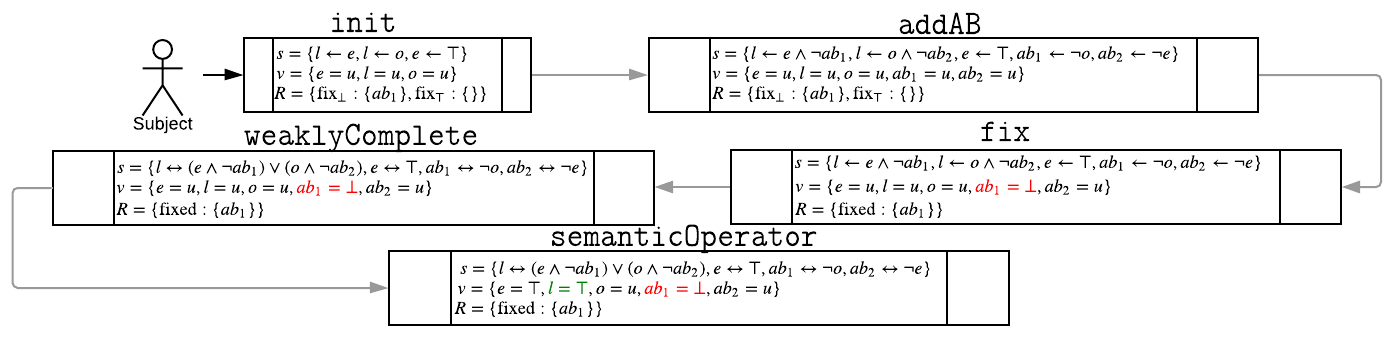
\includegraphics[width=\linewidth]{suppressionSCP_mod2}
\end{center}

\caption{The Suppression Task in which the additional operation of fixing the variable $ab_1$ to false occurs.}
\label{fig:supmod2}
\end{figure*}

The second case of a potential complex operation to add to the search space of our SCPs is the idea of Variable Fixing. The idea that some  conclusions can be fixed \textit{a priori}. Consider a person who strongly doubts the effectiveness of vaccines, we will call her Karen. Karen started her day convinced that giving her child the MMR vaccine is more dangerous than the disease itself. Later that day Karen spoke to her doctor who strongly advised that she vaccinate her child. He offered her a variety of peer-reviewed papers and studies that showed the relative safety of the vaccination. Karen listened carefully to the trained medical professional, and then went home. After some thought Karen decided that he was wrong, and her opinion on vaccines didn't change.

In this example Karen shows a very powerful type of cognitive bias, the unwillingness to change her opinions, despite powerful evidence to the contrary. This phenomenon has been observed across a great many fields of study, from medical psychology \citep{brown2010omission} \citep{wroe2005feeling} to political sciences\citep{tappin2017heart}. In the context of cognitive modelling with logics, it indicates that some mental rules or variables are immutable, regardless of new evidence or valid beliefs that would logically contradict them. Non-monotonic logics, as a class, are already capable of dealing with bias effects, as non-monotonic logics are built on the basis of a preference operation.

 As one possible implementation of this idea, let us introduce a cognitive operation called \texttt{fix}. Fix takes as input any state point and is applicable for any ground point $\bar{p}$ with variable list $V \in \bar{p}$ and categorization variable $R$ with ($fix_\top \lor fix_\bot) \in R$. For all variables $v$ such that $(v \in V) \cap (v \in fix_\top)$ set the value of $v$ to $\top$, For all variables $v$ $(v \in V) \cap (v \in fix_\bot)$ set the value of $v$ to $\bot$. Then remove $fix_\top$ and $fix_\bot$ from $R$. Append $fixed:V_{fix}$ to $R$, where $V_{fix}$ is the set of all variables fixed in this way.

Now, because \texttt{semanticOperator} does not change the values of variables mentioned in $V_{fix} \in fixed:V_{fix}$, $fixed \in R$, Figure~\ref{fig:supmod2} shows the effect of adding a complex operation which fixes the value of the abnormality to false in $v$ so that, no matter what rules in $KB$ when the semantic operator is applied, $ab_1$ will remain false.

\section{Conclusions and Future Work} \label{sec:conc}
SCPs represent a novel and powerful framework for modelling non-monotonic logics. They have been shown capable of modelling the Suppression Task under the WCS for both general and individual cases. SCPs provide a dynamic framework incorporating cognitive operations which are applicable across different logics, provided that those logics share structural features in the initial epistemic state that are compatible with some subset of the known set of cognitive operations. Because the input and output epistemic states need not be structurally similar, SCPs may represent the first approach to modelling human cognition that is able to integrate multiple non-monotonic logic frameworks at run-time and at search-time. 



The addition of two distinct search paradigms to SCPs may one day enable researchers to generate or test hundreds of thousands of models where only the initial epistemic state is known. The first search type, \textit{De Novo Search}, involves finding an SCP that satisfies a goal condition from scratch, iterating over the set of cognitive operations in $M$. This search is important for producing a computationally valid explanation for the general (most common) results of a cognitive task. \textit{Insertion Search}, by contrast, will require finding which additional complex operations can be added to an existing SCP to produce results consistent with the deviant reasoner. This search is important for describing unusual results as deviations from the general reasoner. It is also important for scoring the likelihood of these with respect to the original SCP. Finally, some form of scoring criteria is needed to compare SCPs to one another and evaluate their relative plausibility with respect to the known complexity of the cognitive operations involved. A modified version of Needleman-Wunsch algorithm for string matching has already been theoretically described and must now be implemented in order to determine how similar different models are to each other.

SCPs represent a new frontier for Cognitive Modelling in non-monotonic logics and research into their capabilities and limitations may help create more robust and mathematically consistent explanations and predictions for human behaviour across an extensive array of cognitive tasks.

\section*{Acknowledgments}
Special thanks to Marco Ragni, for his enthusiastic supervision of my ongoing academic studies; Raymond Ind and Sally Magliolo for their help in proof-reading this paper; and to Anastasia Sushich for her tireless support.

\bibliography{bibl}


\section*{Appendix}

\subsection*{Implementations}
An existing Python 3 implementation of the SCP framework (available at \url{https://github.com/AxelInd/SCP_Implementation})  has been able to model experiments related to the Suppression Task and the Wason Selection Task for both general and individual case reasoners using both the WCS and Reiter's Default Logic.

\subsection*{Systematically Adding Abnormalities} \label{ssec:addAbnormalities}
Adding abnormalities is a poorly described process and often relies on intuitionist views of what actually constitutes an abnormal situation. For this reason we have provided one concrete method for adding abnormalities to a logic program (though many others exist and can be extended at will). This particular one is based on the principle that if a variable $v_1$ has the power to make another variable $v_2$ true, then it may be the case that participants believe that any other variables $V'$ satisfying $v_2$ may only do so when $v_1$ holds. This intuition is counter to classical logic, but follows intuitively in cases like the Suppression Task where participants believe that the library not being open may be the reason that the she doesn't study late in the library, even when she has an essay to write. 

In the case of SCPs, the procedure for creating abnormalities is handled by a single complex epistemic operation and so may be substituted for any competing method without disrupting the flow of the SCP. The precise procedure followed for both the WCS and SCP formulation is given by Algorithm~\ref{alg:addAbnormalities}.


\begin{algorithm}
\begin{algorithmic}
\Function{addAbnormalities}{P}
\State \texttt{$P':=[]$}
\For{\texttt{Unique $head$ with $(body \rightarrow head) \in P$}}
\State \texttt{$headDeps$:= [all non-ground bodies s.t.$(body \rightarrow head) \in P$]}
\For{\texttt{$body_i$ with $(body \rightarrow head) \in P$}}
\State \texttt{$ab_{x}$:=new abnormality} \Comment{Where $x$ is a unique identifier}
\State \texttt{create new rule $head \leftarrow body_i \land \lnot ab_x$} 
\State \texttt {$abDeps$:= $headDeps\backslash body_i$} \Comment{$\bot$ if it would be empty}
\State \texttt{$rule$=create new rule $(ab_x \leftarrow dep_1 \land ... \land dep_n)$ for $dep \in abDeps$}
\State $P'+=rule$
\EndFor
\EndFor
\State \Return $P'$
\EndFunction
\end{algorithmic}
\caption{One systematic way to add abnormalities to a logic program.}
\label{alg:addAbnormalities}
\end{algorithm}


\end{document}
